\documentclass{article}
\usepackage{graphicx} % Required for inserting images

\title{PS6 Dunkleberger}
\author{Davis Dunkleberger}
\date{March 2023}

\begin{document}

\maketitle

\section{Cleaning/Transforming Data}
\begin{enumerate}
    \item I chose to use play by play data from the R package hockeyR to create my three visualizations. This packages scrapes play by play data from the internet for nerds like me to use. I filtered the play by play data to account for only plays where goals were scored for my first and third visualizations. I filtered by plays where goals were scored and counted who scored, what team they are one, how many goals that player has scored, and some more advanced stats. This resulted in a table that I used for those two visualizations. 
\end{enumerate}
\section{Visualization 1}

\begin{figure}[h]
    \centering
    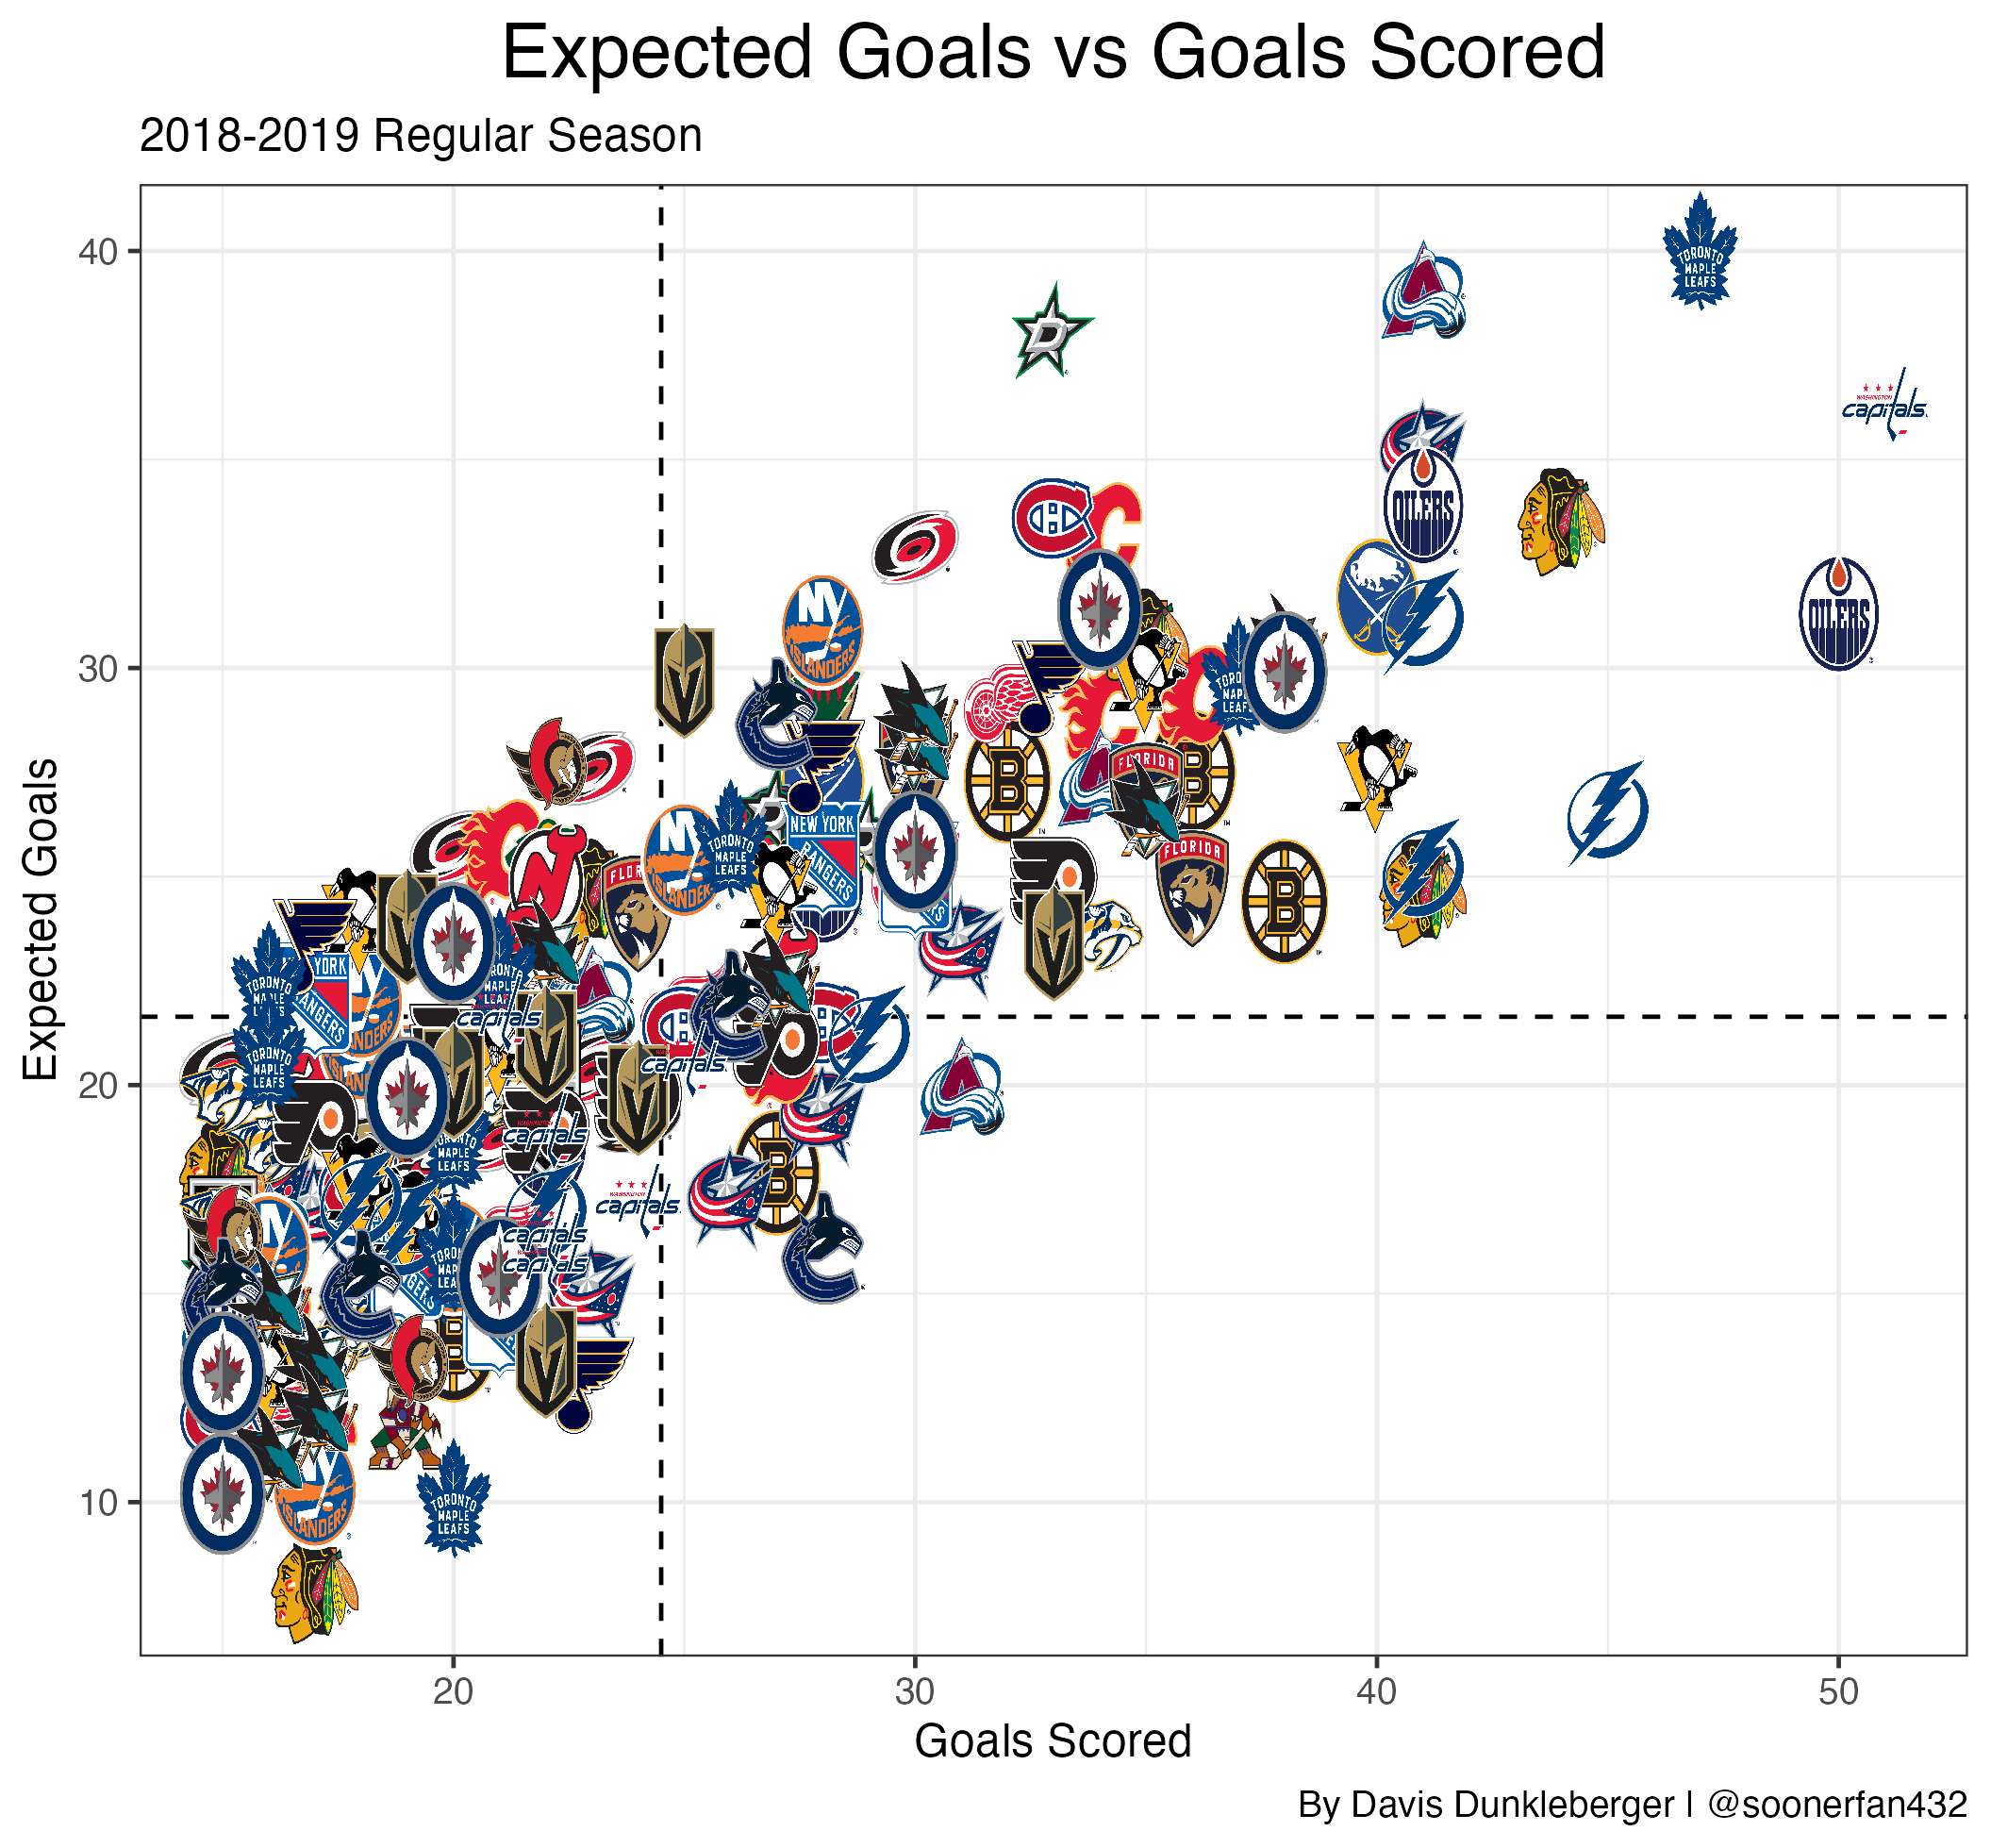
\includegraphics[width = 0.6\textwidth]{Figures/PS6a_Dunkleberger.png}
    \caption{NHL Expected Goals vs Goals Scored, 2018-2019 Regular Season}
    \label{fig:NHL 18-19 EG vs GS}
\end{figure}

\begin{enumerate}
    \item This visualization shows expected goals and the goals scored by certain players during the 2018-2019 regular season. One caveat is that the player must have scored at least 15 goals to be present in this visualization. The logos represent what team the skater played for that season. One limitation is it does not tell you which player is which. I am looking into how to make that happen in future testing. I want the player name and team logo to be present on the visualization. This helps me understand how skaters are performing compared to what they could be expected to do. It helps show what players are performing well or who is not getting any puck luck. It helps provide a comparison to previous seasons and if that player can hold that level of production between seasons. 
\end{enumerate}

\section{Visualization 2}

\begin{figure}[h]
    \centering
    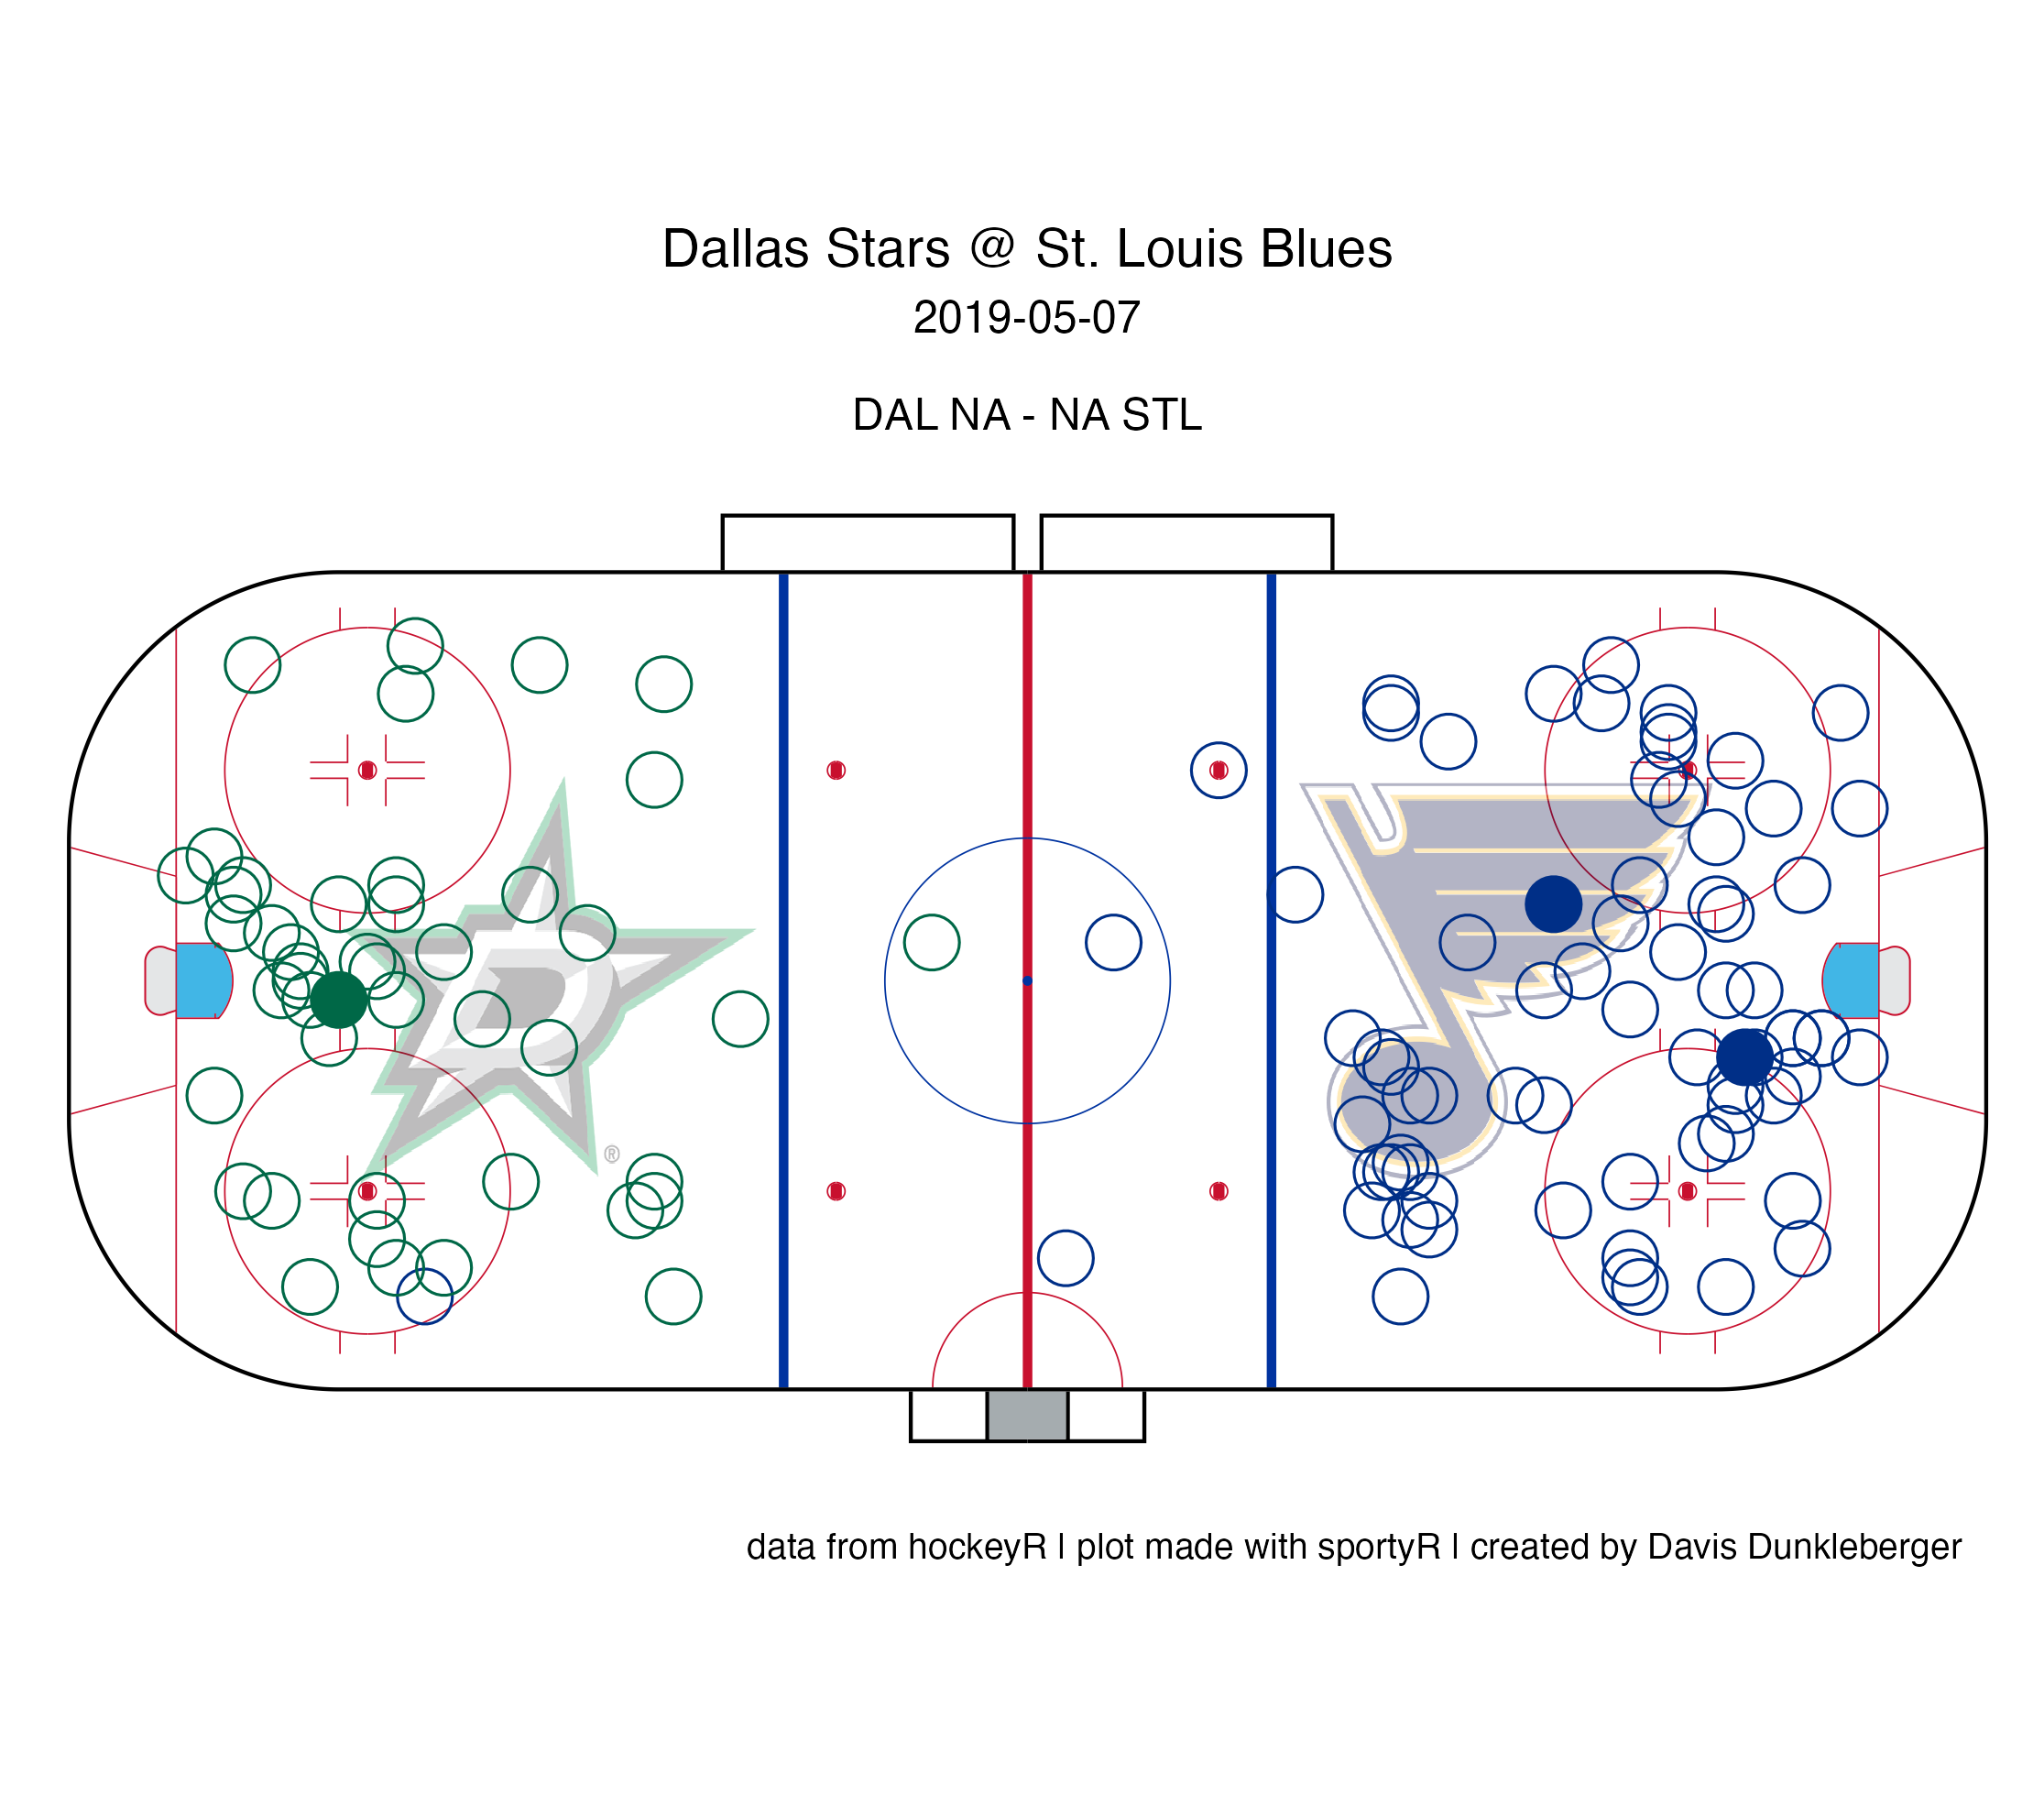
\includegraphics[width = 0.6\textwidth]{Figures/PS6b_Dunkleberger.png}
    \caption{Shot Chart for 2019 WCSF G7}
    \label{fig:Shot Chart for 2019 WCSF Game 7}
\end{figure}

\begin{enumerate}
    \item This figure is demonstrating where shots on goal are registered in a NHL game. The clear dots are shots on goal and the filled ones are goals. This visualization helps me understand where some goals are scored from and who controlled the play. Shots on goal (SOG) are a very simple measurement that are often used to diagnose who performed better. Shots closer to the net are more dangerous than those further away. Shots on goal by itself is just a counting statistic which is not a great measurement by itself; however, the visual aspect of seeing where shots are recorded helps me understand why games could have resulted in the way they did. Of course, this is hockey and variance is a huge part of the game. 
\end{enumerate}

\section{Visualization 3}

\begin{figure}[h]
    \centering
    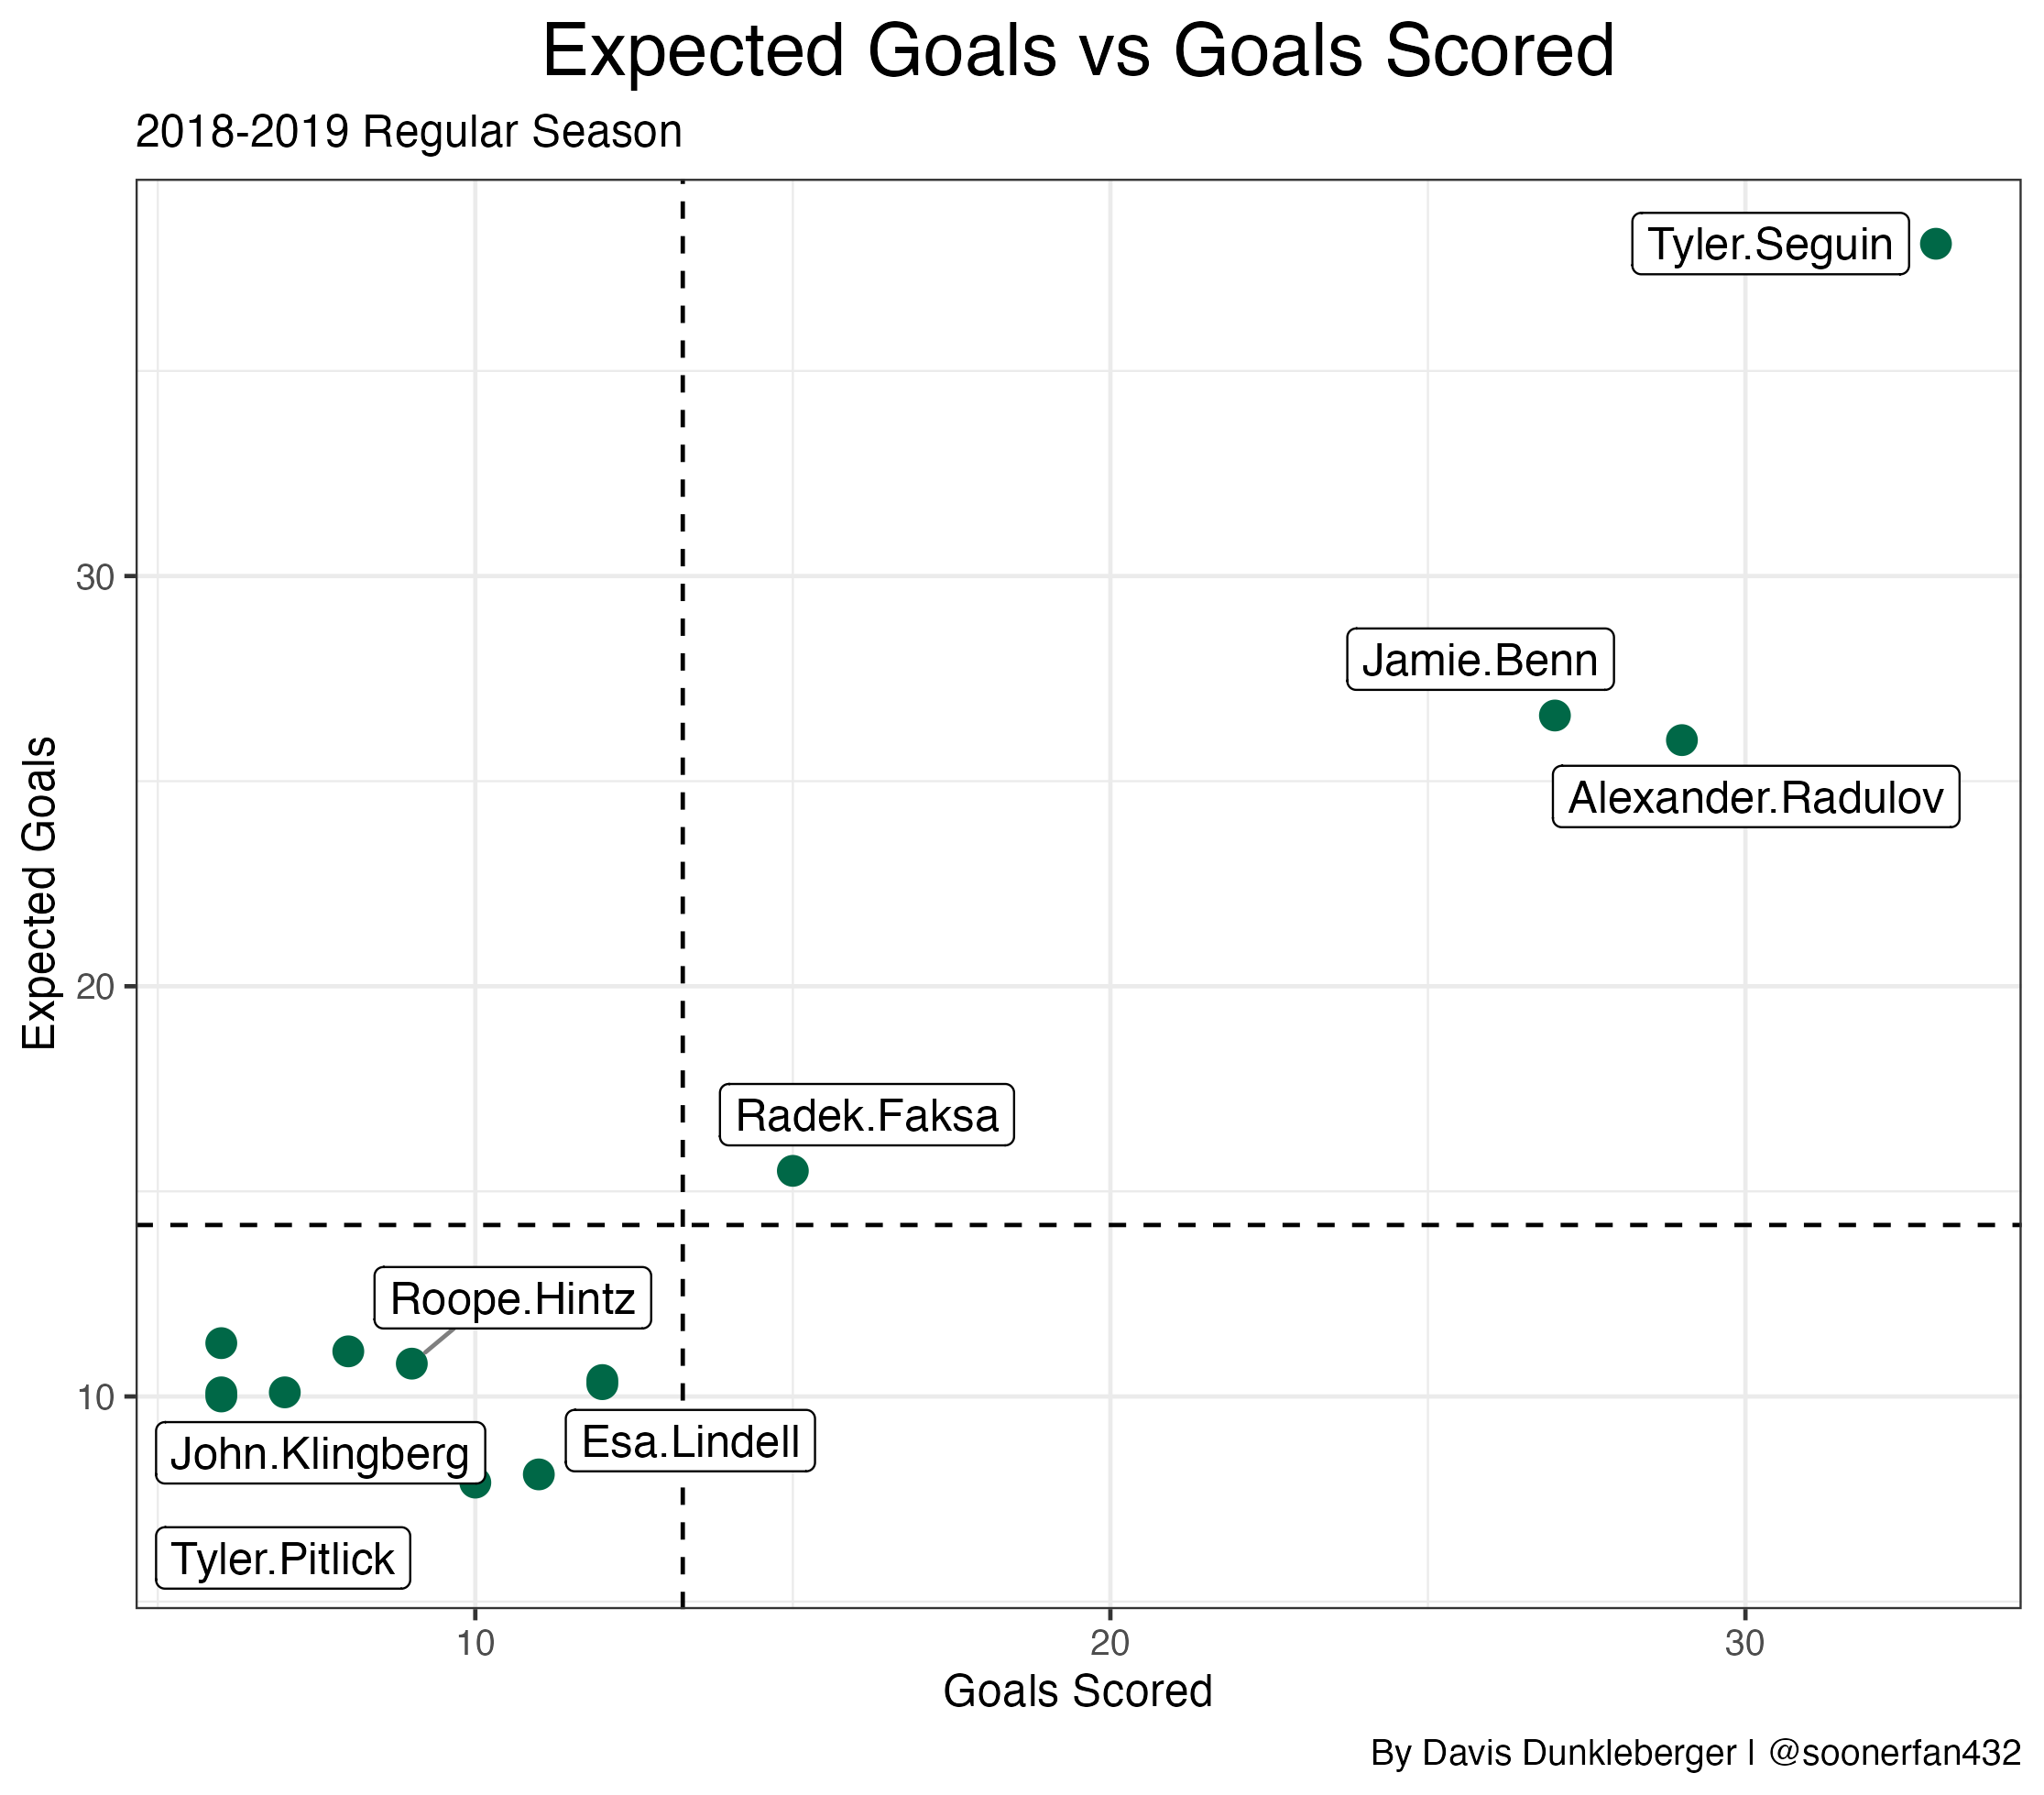
\includegraphics[width = 0.6\textwidth]{Figures/PS6c_Dunkleberger.png}
    \caption{2018-2019 Dallas Stars Expected Goals vs Goals Scored}
    \label{fig:2018-2019 Dallas Stars EG vs GS}
\end{figure}

\begin{enumerate}
    \item This visualization is similar to the first one as it shows the expected goals versus goals scored for one specific team. This chart shows how each player performed that season. This time to be counted in the graph, a player must have scored 5 goals during the regular season. It can help front office decision makers evaluate players season to season. The visualization helps show how teams could be lucky or good. This can be generalized out to other teams and evaluate the luck aspect of their game.
\end{enumerate}

\end{document}
